\begin{exercises} 

\item \label{Ez:9.7.1}    Compute the derivative of each of the following functions in two different ways:  (1) use the rules provided in the theorem stated just after Activity~\ref{A:9.7.2}, and (2) rewrite each given function so that it is stated as a single function (either a scalar function or a vector-valued function with three components), and differentiate component-wise.  Compare your answers to ensure that they are the same.
    \ba
    \item $\ds \vr(t) = \sin(t) \langle 2t, t^2, \arctan(t) \rangle$

    \item $\ds \vs(t) = \vr(2^t)$, where $\vr(t) = \langle t+2, \ln(t), 1 \rangle$.
    
    \item $\ds \vr(t) = \langle \cos(t), \sin(t), t \rangle \cdot \langle -\sin(t), \cos(t), 1 \rangle$
    
    \item $\ds \vr(t) = \langle \cos(t), \sin(t), t \rangle \times \langle -\sin(t), \cos(t), 1 \rangle$
     
    \ea

\begin{exerciseSolution}
    \ba
    \item First we use part 2 of the theorem to find that 
\[\vr'(t) = \sin(t) \left\langle 2, 2t, \frac{1}{1+t^2} \right\rangle + \cos(t) \langle 2t, t^2, \arctan(t) \rangle.\]
Next we write $\vr(t)$ as a vector-valued function with three components:
\[\vr(t) = \langle 2t \sin(t), t^2 \sin(t), \arctan(t) \sin(t) \rangle.\]
Then we differentiate component-wise to obtain
\[\frac{d}{dt} \vr(t)  = \left\langle 2\sin(t) + 2t \cos(t), 2t \sin(t) + t^2 \cos(t), \frac{1}{1+t^2} \sin(t) + \arctan(t) \cos(t) \right\rangle.\]

    \item First we use part 5 of the theorem to calculate
\[\vs'(t) = \vr'(2^t)(2^t \ln(2)) = 2^t \ln(2) \left\langle 1, \frac{1}{2^t}, 0 \right\rangle.\]
Next we write $\vs(t)$ as a vector-valued function with three components and differentiate component-wise to obtain
\[\frac{d}{dt} \langle 2^t+2, \ln(2^t), 1 \rangle = \left\langle 2^t \ln(2), \ln(2), 0 \right\rangle.\]
    
    \item First we use part 3 of the theorem to calculate
\[\vr'(t) = \langle -\sin(t), \cos(t), 1 \rangle \cdot \langle -\sin(t), \cos(t), 1 \rangle + \langle \cos(t), \sin(t), t \rangle \cdot \langle -\cos(t), -\sin(t), 0 \rangle.\]
Next we write $\vr(t)$ as a vector-valued function with three components and differentiate component-wise to obtain
\[\frac{d}{dt} \langle -\cos(t) \sin(t), \sin(t) \cos(t), t \rangle = \langle -(\cos^2(t)-\sin^2(t)), \cos^2(t)-\sin^2(t), 1 \rangle.\]
    
    \item First we use part 4 of the theorem and see that 
\[\vr'(t) = \langle -\sin(t), \cos(t), 1 \rangle \times \langle -\sin(t), \cos(t), 1 \rangle + \langle \cos(t), \sin(t), t \rangle \times \langle -\cos(t), -\sin(t), 0 \rangle = \langle t \sin(t), -t\cos(t), 0 \rangle.\]
Next we write $\vr(t)$ as a vector-valued function with three components and differentiate component-wise to obtain
\begin{align*}
\frac{d}{dt} \langle \sin(t)-t\cos(t), -\cos(t)-t\sin(t), 1 \rangle &= \langle \cos(t) - (\cos(t)-t\sin(t)), \sin(t)-(\sin(t)+t\cos(t)), 0 \rangle \\
	&= \langle t \sin(t), -t\cos(t), 0 \rangle.
\end{align*}
     
    \ea
\end{exerciseSolution}


\item \label{Ez:9.7.2}   Consider the two vector-valued functions given by 
$$\vr(t) = \left\langle t + 1, \cos\left(\frac{\pi}{2} t\right), \frac{1}{1+t} \right\rangle$$
and
$$\vw(s) = \left\langle s^2, \sin\left(\frac{\pi}{2}s\right), s \right\rangle.$$ 

%\begin{figure}[h]
%\begin{center}
 %\includegraphics{figures/1_1_Ez1.eps}
 %\caption{A bungee jumper's height function.} \label{F:1.1.Ez1}
%\end{center}
%\end{figure}

\ba

	\item Determine the point of intersection of the curves generated by $\vr(t)$ and $\vw(s)$.  To do so, you will have to find values of $a$ and $b$ that result in $\vr(a)$ and $\vw(b)$ being the same vector.
	
	\item Use the value of $a$ you determined in (a) to find a vector form of the tangent line to $\vr(t)$ at the point where $t = a$.
	
	\item Use the value of $b$ you determined in (a) to find a vector form of the tangent line to $\vw(s)$ at the point where $s = b$.
	
	\item Suppose that $z = f(x,y)$ is a function that generates a surface in three-dimensional space, and that the curves generated by $\vr(t)$ and $\vw(s)$ both lie on this surface.  Note particularly that the point of intersection you found in (a) lies on this surface.  In addition, observe that the two tangent lines found in (b) and (c) both lie in the tangent plane to the surface at the point of intersection.  Use your preceding work to determine the equation of this tangent plane.
\ea

\begin{exerciseSolution}
\ba

	\item We will need to find values of $a$ and $b$ so that $a+1=b^2$, $\cos\left(\frac{\pi}{2} a\right) = \sin\left(\frac{\pi}{2}b\right)$, and $\frac{1}{1+a} = b$. The first equation tells us that $a = b^2-1$. Substituting into the third equation results in 
\[\frac{1}{1+b^2-1} = \frac{1}{b^2} = b.\]
This equation is satisfied when $b^3=1$ or when $b=1$. This makes $a=0$. Note that the second equation is also satisfied when $a=0$ and $b=1$. So the point of intersection of the curves occurs when $a=0$ and $b=1$, which produces the point $(1, 1,1)$. 
	
	\item A direction vector for this tangent line will be 
\[\vr'(a) = \left\langle 1, -\sin\left(\frac{\pi}{2} (0)\right)\left(\frac{\pi}{2}\right), -\frac{1}{(1+0)^2} \right\rangle = \langle 1,0,-1\rangle.\]
So a vector form of the tangent line to $\vr(t)$ at the point where $t = a$ is
\[\langle 1 + t, 1, 1-t \rangle.\]
	
	\item A direction vector for this tangent line will be 
\[\vw'(b) = \left\langle 2(1), \cos\left(\frac{\pi}{2} (1)\right)\left(\frac{\pi}{2}\right), 1 \right\rangle = \langle 2,0,1\rangle.\]
So a vector form of the tangent line to $\vw(t)$ at the point where $s = b$ is
\[\langle 1 + 2t, 1, 1+t \rangle.\]
	
	\item A normal vector for this tangent plane will be perpendicular to the direction vectors for the two tangent lines. So a normal vector for this tangent plane is 
\[\langle 1, 0, -1 \rangle \times \langle 2, 0, 1 \rangle = \langle 0, -3, 0 \rangle.\]
So the equation of the tangent plane to the surface at $(1,1,1)$ is 
\[-3(y-1) = 0 \text{ or } y=1.\]
\ea
\end{exerciseSolution}



\item \label{Ez:9.7.3}   In this exercise, we determine the equation of a plane tangent to the surface defined by $f(x,y) = \sqrt{x^2+y^2}$ at the point $(3,4,5)$.
    \ba
    \item Find a parameterization for the $x=3$ trace of $f$. What is a direction vector for the line tangent to this trace at the point $(3,4,5)$?

    \item  Find a parameterization for the $y=4$ trace of $f$. What is a direction vector for the line tangent to this trace at the point $(3,4,5)$?

    \item The direction vectors in parts (a) and (b) form a plane containing the point $(3,4,5)$. What is a normal vector for this plane? 
    
    \item Use your work in parts (a), (b), and (c) to deterring an equation for the tangent plane.  Then, use appropriate technology to draw the graph of $f$ and the plane you determined on the same set of axes. What do you observe? (We will discuss tangent planes in more detail in Chapter 10.)

    \ea
\begin{exerciseSolution}
    \ba
    \item A parameterization for the $x=3$ trace of $f$ is
\[\langle 3, t, f(3,t) \rangle = \langle 3,t, \sqrt{t^2+9} \rangle.\]
A direction vector for the line tangent to this trace at the point $(3,4,5)$ is 
\[\frac{d}{dt}\langle 3,t, \sqrt{t^2+9} \rangle\biggm|_{t=4} = \left\langle 0, 1, \frac{1}{2}\frac{2(4)}{\sqrt{4^2+9}} \right\rangle = \left\langle 0, 1, \frac{4}{5} \right\rangle.\]

    \item A parameterization for the $y=4$ trace of $f$ is
\[\langle t, 4, f(t,4) \rangle = \langle t,4, \sqrt{16+t^2} \rangle.\]
A direction vector for the line tangent to this trace at the point $(3,4,5)$ is 
\[\frac{d}{dt}\langle t,4, \sqrt{16+t^2} \rangle\biggm|_{t=3} = \left\langle 1, 0, \frac{1}{2}\frac{2(3)}{\sqrt{16+3^2}} \right\rangle = \left\langle 1, 0, \frac{3}{5} \right\rangle.\]

    \item A normal vector for this plane is 
\[\left\langle 0, 1, \frac{4}{5} \right\rangle \times \left\langle 1, 0, \frac{3}{5} \right\rangle = \left\langle \frac{3}{5}, \frac{4}{5}, -1 \right\rangle.\]
    
    \item An equation for the tangent plane to the surface $f$ at the point $(3,4,5)$ is 
\[\frac{3}{5}(x-3) + \frac{4}{5}(x-4) + (-1)(z-5) = 0\]
or
\[z=\frac{3}{5}(x-3) + \frac{4}{5}(x-4) - 5.\]


    \ea
\end{exerciseSolution}


\item \label{Ez:9.7.4}   For each given function $\vr$, determine $\int \vr(t) \ dt$.  In addition, recalling the Fundamental Theorem of Calculus for functions of a single variable, also evaluate $\int_0^1 \vr(t) \ dt$ for each given function $\vr$.  Is the resulting quantity a scalar or a vector?  What does it measure?


	\ba
	\item $\ds \vr(t) = \left\langle \cos(t), \frac{1}{t+1}, te^t \right\rangle$ 
	
	\item $\ds \vr(t) = \left\langle \cos(3t), \sin(2t), t \right\rangle $ 
	
	\item $\ds \vr(t) = \left\langle \frac{t}{1+t^2}, te^{t^2}, \frac{1}{1+t^2} \right\rangle$ 

	\ea
\begin{exerciseSolution}
	\ba
	\item We integrate component-wise to obtain
\begin{align*}
\int \vr(t) \, dt &= \left\langle \int \cos(t) \, dt, \int \frac{1}{t+1} \, dt, \int te^t \, dt \right\rangle \\
	&= \left\langle \sin(t),  \ln|t+1|, te^t - e^t \right\rangle + \vc.
\end{align*} 
So
\begin{align*}
\int_0^1 \vr(t) \, dt &= \left\langle \sin(t),  \ln|t+1|, te^t - e^t \right\rangle \biggm|_0^1 \\
	&= \langle \sin(1), \ln(2), 0 \rangle - \langle 0, 0, -1 \rangle \\
	&= \langle \sin(1), \ln(2), 1 \rangle.
\end{align*}
If $\vr(t)$ represents the velocity of an object at time $t$, then $\int_0^1 \vr(t) \ dt$ is the total change in position of the object from time $t=0$ to time $t=1$. 
	
	\item We integrate component-wise to obtain
\begin{align*}
\int \vr(t) \, dt &= \left\langle \int \cos(3t) \, dt, \int \sin(2t) \, dt, \int t \, dt \right\rangle \\
	&= \left\langle \frac{1}{3}\sin(3t), -\frac{1}{2} \cos(2t), \frac{1}{2}t^2 \right\rangle + \vc.
\end{align*} 
So
\begin{align*}
\int_0^1 \vr(t) \, dt &= \left\langle \frac{1}{3}\sin(3t), -\frac{1}{2} \cos(2t), \frac{1}{2}t^2 \right\rangle \biggm|_0^1 \\
	&= \left\langle \frac{1}{3}\sin(3), -\frac{1}{2} \cos(2), \frac{1}{2} \right\rangle - \left\langle 0, -\frac{1}{2}, 0 \right\rangle \\
	&= \left\langle \frac{1}{3}\sin(3), -\frac{1}{2} \cos(2)+\frac{1}{2}, \frac{1}{2} \right\rangle .
\end{align*}
	
	\item We integrate component-wise to obtain
\begin{align*}
\int \vr(t) \, dt &= \left\langle \int \frac{t}{1+t^2} \, dt, \int te^{t^2} \, dt, \int \frac{1}{1+t^2} \, dt \right\rangle \\
	&= \left\langle \frac{1}{2}\ln(1+t^2), \frac{1}{2} e^{t^2}, \arctan(t) \right\rangle + \vc.
\end{align*} 
So
\begin{align*}
\int_0^1 \vr(t) \, dt &= \left\langle \frac{1}{2}\ln(1+t^2), \frac{1}{2} e^{t^2}, \arctan(t) \right\rangle \biggm|_0^1 \\
	&= \left\langle \frac{1}{2}\ln(2), \frac{1}{2} e, \arctan(1) \right\rangle - \left\langle 0, \frac{1}{2}, \arctan(0) \right\rangle \\
	&= \left\langle \frac{1}{2}\ln(2), \frac{1}{2} e - \frac{1}{2}, \frac{\pi}{4} \right\rangle.
\end{align*}

	\ea
\end{exerciseSolution}

\item \label{Ez:9.7.5} In this exercise, we develop the formula for the position function of a projectile that has been launched at an initial speed of $|\vv_0|$ and a launch angle of $\theta.$  Recall that  $\va(t) = \langle 0, -g \rangle$ is the constant acceleration of the projectile at any time $t$.
\ba
    \item Find all velocity vectors for the given acceleration vector $\va$.  When you anti-differentiate, remember that there is an arbitrary constant that arises in each component.

   \item Use the given information about initial speed and launch angle to find $\vv_0$, the initial velocity of the projectile.  You will want to write the vector in terms of its components, which will involve $\sin(\theta)$ and $\cos(\theta)$.

    \item Next, find the specific velocity vector function $\vv(t)$ for the projectile. That is, combine your work in (a) and (b) in order to determine expressions in terms of $|\vv_0|$ and $\theta$ for the constants that arose when integrating.

 \item Find all possible position vectors for the velocity vector $\vv(t)$ you determined in (c).

    \item Let $\vr(t)$ denote the position vector function for the given projectile. Use the fact that the object is fired from the position $(x_0, y_0)$ to show it follows that
\[\vr(t) = \left\langle |\vv_0| \cos(\theta)t + x_0, -\frac{g}{2}t^2 + |\vv_0| \sin(\theta)t + y_0 \right\rangle.\]

    \ea

\begin{exerciseSolution}
\ba
    \item Integrating the acceleration vector gives us the family of velocity functions
\[\vv(t) = \int \va(t) \, dt = \langle 0, -gt \rangle + \vc,\]
where $\vc$ is some constant vector.

   \item An application of trigonometry shows that $\vv_0 = \langle |\vv_0| \cos(\theta), |\vv_0| \sin(\theta) \rangle$. 

    \item Note that 
\[\langle |\vv_0| \cos(\theta), |\vv_0| \sin(\theta) \rangle = \vv_(0) = \langle 0, (-g)(0) \rangle + \vc,\]
so 
\[\vc = \langle |\vv_0| \cos(\theta), |\vv_0| \sin(\theta) \rangle.\]
Thus,
\[\vv(t) =  \langle |\vv_0| \cos(\theta), -gt + |\vv_0| \sin(\theta) \rangle.\]

 \item If $\vr$ is the vector-valued function that gives the position of the object at time $t$, then
\[\vr(t) = \int \vv(t) \, dt = \left\langle |\vv_0| \cos(\theta)t, -g\frac{t^2}{2} + |\vv_0| \sin(\theta)t \right\rangle + \vk,\]
where $\vk$ is some constant vector.

    \item Now $\vr(0) = \langle x_0, y_0 \rangle$, so we have
\[\langle x_0, y_0 \rangle =  \langle |\vv_0| \cos(\theta)(0), -g\frac{0^2}{2} + |\vv_0| \sin(\theta)(0) \rangle + \vk\]
and
\[\vk = \langle x_0, y_0 \rangle.\]
We conclude that
\[\vr(t) = \langle |\vv_0| \cos(\theta)t + x_0, -g\frac{t^2}{2} + |\vv_0| \sin(\theta)t + y_0 \rangle.\]
\ea
\end{exerciseSolution}

\item \label{Ez:9.7.6} A {\em central force} is one that
  acts on an object so that the force $\vF$ is parallel to the
  object's position $\vr$.  Since Newton's Second Law says that an
  object's acceleration is proportional to the force exerted on it,
  the acceleration $\va$ of an object moving under a central force
  will be parallel to its position $\vr$.  For instance, the Earth's
  acceleration due to the 
  gravitational force that the sun exerts on the Earth is parallel to
  the Earth's position vector as shown in Figure \ref{F:9.7.sun}.

\begin{figure}[ht]
  \begin{center}
    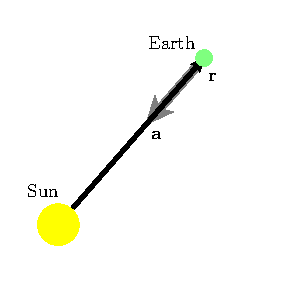
\includegraphics{figures/fig_9_7_sun.eps}
    \caption{A central force.}
    \label{F:9.7.sun}
  \end{center}
\end{figure}

\ba
\item If an object of mass $m$ is moving under a central force, 
  the angular momentum vector is defined to be $\vL=m\vr\times\vv$.
  Assuming the mass is constant, show that the angular momentum is
  constant by showing that
  $$
  \frac{d\vL}{dt} = \vzero.
  $$

\item Explain why $\vL\cdot\vr = 0$.

\item Explain why we may conclude that the object is constrained to
  lie in the plane passing through the origin and perpendicular to
  $\vL$.

\ea

\begin{exerciseSolution}
\ba
\item Since the acceleration is parallel to the position under a central force, if follows that $\vr \times \va = \vzero$. By the product rule we have that 
\begin{align*}
\frac{d\vL}{dt} &= \frac{d}{dt} m\vr\times\vv \\
	&= (m\vr \times \vv') + (m\vr' \times \vv)  \\
	&= m(\vr \times \va) + m(\vv \times \vv) \\
	&= \vzero.
\end{align*}
Since the derivative of $\vL$ is $\vzero$, it follows that $\vL$ is constant. 
  

\item Recall that the cross product of two vectors is perpendicular to both vectors, so $\vL = m(\vr\times\vv)$ is perpendicular to $\vr$. Thus, $\vL\cdot\vr = 0$.

\item Since $\vL = m(\vr \times \vv$ is constant, the position and velocity vectors lie in a single plane perpendicular to $\vL$. To the objects position and motion are constrained to lie in the plane passing through the origin and perpendicular to $\vL$.

\ea
\end{exerciseSolution}


\end{exercises}
\afterexercises
